\documentclass[letterpaper,12pt]{report}
\usepackage[top=1in, bottom=1in, left=1in, right=1in]{geometry}
\usepackage{fancyhdr,tocloft,natbib,url,graphicx,float,listings,sidecap,wrapfig}
\usepackage[font=small,labelfont=bf,labelsep=period]{caption}
\usepackage{tabularx}
\usepackage{setspace}
\usepackage{hyperref}
\usepackage[all]{hypcap}
\usepackage{qtree,algorithm,algorithmic}
\usepackage{natbib}
\pagestyle{plain}
\fancyhf{}
\lhead{}
\chead{}
\rhead{}
\cfoot{\thepage}

%\floatstyle{boxed}
%\restylefloat{figure}

\hypersetup {
	colorlinks=false,
	pdfborder={0 0 0},
}

\setcounter{secnumdepth}{3}
\renewcommand*\thesection{\arabic{section}.}
\renewcommand*\thesubsection{\thesection \arabic{subsection}.}
\renewcommand*\thesubsubsection{\thesubsection \arabic{subsubsection}.}

\setcounter{tocdepth}{3}
\renewcommand\contentsname{}				% TOC title
\renewcommand\listfigurename{}				% LOF title
\renewcommand\listtablename{}				% LOT title
\setlength\cftaftertoctitleskip{-0.5in}
\setlength\cftafterloftitleskip{-0.5in}
\setlength\cftafterlottitleskip{-0.5in}

\renewcommand\bibsection{\section{References}}

\begin{document}

\hypersetup{pageanchor=false}
%%  COVER PAGE
\begin{titlepage}
	\begin{center}
		\vspace*{0.5in}
		\begin{doublespace}
			\LARGE \textbf{NeuraViz: A Web Application For Visualizing Artificial Neural Network Structures} \\
			\vspace*{1in}
			\normalsize
			A Manuscript \\
			Submitted to \\
			the Department of Computer Science \\
			and the Faculty of the\\
			University of Wisconsin--La Crosse \\
			La Crosse, Wisconsin \\
			\vspace*{0.5in}
			by \\
			\large
			\textbf{Bennett Wendorf} \\

			\vspace*{0.5in}
			\normalsize
			in Partial Fulfillment of the \\
			Requirements for the Degree of\\
			\Large{\textbf{Master of Software Engineering}} \\
			\normalsize
			May, 2024
		\end{doublespace}
	\end{center}
\end{titlepage}
	
\clearpage

%% SIGNATURE PAGE
\thispagestyle{empty}
\vspace*{0.3in}
\begin{center}
	\large{\textbf{NeuraViz: A Web Application For Visualizing Artificial Neural Network Structures}} \\
	\vspace{0.75in}
	\normalsize{By Bennett Wendorf}
\end{center}

\vspace{0.5in}
\noindent We recommend acceptance of this manuscript in partial fulfillment of this candidate's requirements for the degree of Master of Software Engineering in Computer Science. The candidate has completed the oral examination requirement of the capstone project for the degree. \\

\noindent
\begin{tabularx}{\textwidth}{p{3in}Xp{2in}} % TODO: Add committee members
	\rule{0pt}{50pt} & & \\
	\hrulefill & & \hrulefill \\
	Prof.\ Albert Einstein & & Date \\
	Examination Committee Chairperson & & \\
	\rule{0pt}{50pt} & & \\
	\hrulefill & & \hrulefill \\
	Prof.\ Isaac Newton & & Date \\
	Examination Committee Member & & \\
	\rule{0pt}{50pt} & & \\
	\hrulefill & & \hrulefill \\
	Prof.\ Marie Curie & & Date \\
	Examination Committee Member & & \\
\end{tabularx}


\clearpage

\hypersetup{pageanchor=true}
\setcounter{page}{1}
\pagenumbering{roman}
\renewcommand\arraystretch{1.5}

%% ABSTRACT
\section*{Abstract}
\addcontentsline{toc}{section}{Abstract} % TODO: Add abstract
Wendorf, Bennett, ``NeuraViz: A Web Application For Visualizing Artificial Neural Network Structures,'' Master of Software Engineering, May 2024, (Jason Sauppe, Ph.D.). \\

This manuscript describes the software engineering processes and principles adhered to during the development of Neuraviz, a web application for visualizing artificial neural network structures. Users upload pre-trained machine learning models from popular frameworks including Pytorch and Keras, and Neuraviz generates a visual representation of the model's architecture. The following manuscript focuses on the design, implementation, testing, and deployment of NeuraViz in an effort to comprehensively encapsulate the entire development process.
\clearpage

%%% ACKNOWLEDGEMENTS
\section*{Acknowledgements}
\addcontentsline{toc}{section}{Acknowledgments}
I would like to extend my sincerest thanks to my project advisor, Dr. Jason Sauppe, for his guidance and support throughout the development of NeuraViz. His feedback was always crucial in pointing me in the right direction, especially when I was overwhelmed with possibilities. 

Thank you also to the entire computer science department at the University of Wisconsin-La Crosse for tirelessly helping me through all my coursework and projects throughout my tenure at the university. My ability to complete this monumental task would not have been possible without them.

I would also like to thank the open source community for providing the tools and resources used in this project. Open source software is an integral part of the modern software space and none of our lives would be the same without it.

Finally, I would like to thank my parents, family, friends, and all the teachers, mentors, and colleagues who have helped, supported, and encouraged me throughout my life. I am more grateful thank I can possibly express in words.
\clearpage

%% TABLE OF CONTENTS
\section*{Table of Contents}
\tableofcontents
\clearpage


%% LIST OF TABLES
\section*{List of Tables}
\addcontentsline{toc}{section}{List of Tables}
\listoftables
\clearpage

%% LIST OF FIGURES
\section*{List of Figures}
\addcontentsline{toc}{section}{List of Figures}
\listoffigures
\clearpage

%% GLOSSARY
\section*{Glossary}
\addcontentsline{toc}{section}{Glossary}
\subsection*{Artificial Neural Network}
A computational model that is inspired by the way biological neural networks in the human brain process information. It is composed of layers of nodes, each of which is connected to the next layer via links. Each connection has a weight associated with it, and the network learns by adjusting these weights based on the input data. The network can be trained to recognize patterns in data, make predictions, and perform other tasks.

\subsection*{Activation Function}
A function that determines the output of a node in a neural network based on the weighted sum of its inputs. Common activation functions include the sigmoid function, the hyperbolic tangent function, and the rectified linear unit (ReLU) function. The activation function introduces non-linearity into the network, allowing it to learn complex patterns in the data.

\subsection*{\LaTeX{}}
\LaTeX{} is a document markup language for the TeX typesetting program.

\subsection*{TikZ}
TikZ is a graph drawing package for \LaTeX{} that allows users to create high-quality diagrams and illustrations.

\subsection*{Scalable Vector Graphics (SVG)}
SVG is an XML-based vector image format for two-dimensional graphics with support for interactivity and animation. It is commonly used in web applications.

\subsection*{Raster Graphics}
Raster graphics are digital images composed of a grid of pixels. Each pixel has a specific color value, and the image is displayed by rendering the pixels on a screen. Common raster graphics formats include JPEG, PNG, and GIF.

\subsection*{Python}
Python is a high-level programming language known for its simplicity and readability. It is widely used in data science, machine learning, web development, and other fields.

\subsection*{PyTorch}
PyTorch is a popular open-source machine learning library for building artificial neural networks. It is known for its flexibility and ease of use, making it a popular choice for researchers and developers.

\subsection*{Keras}
Keras is an open-source deep learning library written in Python that provides a high-level interface for building and training neural networks. Distributed by the Tensorflow team, it is a high-level API on top of Tensorflow and other popular frameworks.

\subsection*{TypeScript}
TypeScript is a superset of JavaScript that adds static typing and other features to the language. It is commonly used in web development to improve code quality and maintainability.

\subsection*{Parsing}
Parsing is the process of analyzing a sequence of symbols to determine its grammatical structure. In the context of this project, it refers to the process of extracting information from a machine learning model object to generate a visual representation of the model's architecture.

\subsection*{Sprint}
A sprint is a short, time-boxed period during which a development team works to complete a set amount of work. Sprints are a key component of the Scrum agile framework and are typically 1-4 weeks long.

\subsection*{JavaScript Object Notation (JSON)}
JSON is a lightweight data interchange format that is easy for humans to read and write and easy for machines to parse and generate. It is commonly used to transmit data between a server and a web application.
\clearpage

\setcounter{page}{1}
\pagenumbering{arabic}

\IfFileExists{01_introduction/introduction}{\section{Introduction}
\label{sec:Introduction}

\subsection{Overview} 
This project aims to develop a software system to visualize the architecture of artificial neural networks. Neural networks (NNs) are a class of machine learning models that are inspired by the structure and function of the human brain. They are composed of a large number of interconnected processing elements, called neurons, which work together to solve complex problems. The architecture of a neural network refers to the arrangement of neurons and the connections between them. In addition to the general structure of a network, the weights and biases that control its function can provide useful insight into the inner workings of the model. The final integral parts of the neural network architecture are the activation functions that govern how data propagates through the network. Visualizing the architecture of a neural network can help students and researchers understand the structure of the model, identify potential issues, and communicate the model to others. 
% TODO: Consider linking to external resources for neural network information

This project will develop a web application that allows users to upload pre-trained neural network models and generate visual representations of their architecture. The application will support models trained using popular machine learning frameworks such as PyTorch and Keras. The resulting graph structure will be visualized in a pannable and zoomable svg format that shows the ordering of neurons, biases on those neurons, the weights of the connections between them and activation functions on each layer.
% TODO: Consider adding examples of what these architectures might look like

The application will be designed to be user-friendly and accessible to a wide range of users, including students and researchers. It will be implemented using modern web technologies and will be deployed as a web service that can be accessed from any device with an internet connection. The project will follow best practices in software engineering, including requirements analysis, design, implementation, testing, and deployment. The resulting application will be a valuable tool for anyone working with neural networks, but will be primarily targeted toward post-secondary educational students learning about machine learning and neural networks for the first time.

\subsection{Background}
Neural networks are a notoriously difficult concept to understand, especially for those who are newer to the field of machine learning. The architecture of a neural network is a key component of understanding how the model functions, but it can be difficult to visualize and comprehend. There are a handful to tools available for visualizing neural network architectures, but they are often limited in their scope. For example, Google's TensorBoard is a popular tool, but only natively supports TensorFlow and Keras models. In researching existing tools such as TensorBoard, Netron, and ENNUI, it was found that none of them supported the same range of formats as NeuraViz. This project aims to develop a user-friendly tool that is accessible to a wide range of users, including students and researchers who are new to the field of machine learning, and to support a wider range of model formats than other offerings.

\subsection{Goals}
NeuraViz is designed specifically with user-friendliness and simplicity in mind. The minimal interface focuses on the visualizes of the neural networks themselves, with minimal distractions. The use of color and shape in the visualizations will help to make the network architecture more understandable at a glance, quickly identifying neurons and connections that are the most important. Where needed, users can also zoom in or out an click on elements to see more detailed information.

Portability is another key goal of the development. Modern web technologies ensure the application is accessible from a range of devices, though it is most optimized for a desktop or laptop experience. Since the application is deployed as a web application, users don't need to install software on their own machines, or even sign in to be able to use the tool. To enhance this ability further, graph representations can also be exported as raw SVG or in tikz format for use within LaTeX documents. 
}{}\clearpage
\IfFileExists{02_dev_process/software_development_process}{\section{Software Development Process}
\label{sec:SoftwareDevelopmentProcess}

\subsection{Overview} 
Developing software is an extensive and complex process that requires a lot of planning, both in relation to the methodologies used during the development process and the functional and non-functional requirements of the software. This section discusses life cycle models considered for NeuraViz's development, the model that was eventually chosen, and modifications to the model that were necessary for the development of this particular system. It also outlines functional and non-functional requirements for NeuraViz.

\subsection{Life Cycle Model}
Prior to beginning development of NeuraViz, a number of software life cycle models were considered to govern the pace and structure of development. In all, the Waterfall model, Iterative model, and Agile model were considered. More specifically with Agile, a variation of Scrum, modified for a single developer, was considered. Ultimately, the modified scrum model was chosen for its flexibility and ability to adapt quickly to changing requirements.

\subsubsection{Waterfall Model}
The waterfall model is one of the oldest software development lifecycle (SDLC) models, originally proposed by Winston Royce in 1970 \cite{Gagan2020}. The model is a linear, sequential approach to software development, with each phase of the development process directly following the previous phase. Each subsequent phase relies on the previous phase, and as such the model does not allow going back to previous phases once they are completed. The first phase of the waterfall model is the requirement analysis phase, in which project requirements, both functional and non-functional, are gathered and documented. At this phase, requirements are also often analyzed for traits like consistency and feasibility. The second phase is the system design phase, in which the architecture of the software system is designed in full. All details of what needs to be done and how it will be completed are considered and documented during this phase. Third, the implementation phase is where the code for the software is written and the design from the previous step is implemented in full, exactly as specified during the design phase. During the fourth phase, the software is tested for bugs and errors, and issues are resolved as needed. Fifth, the software is deployed to the client in its entirety. In the waterfall model, this is the first time the client has seen the software. Finally, the software is maintained and updated as needed for as long as the client needs it. Figure \ref{fig:waterfall_model} shows a diagram of the waterfall model and its constituent parts.

\begin{figure}[htb]
    \centering
    \includesvg[width=.75\textwidth]{02_dev_process/res/waterfall_model.svg}
    \caption[Waterfall Model Diagram]{Waterfall Model Diagram (recreated from \cite{tutorialspoint})}
    \label{fig:waterfall_model}
\end{figure}

Because of its rigid structure, the waterfall model excels at being very easy to understand and pick up quickly for new developers, which was initially intriguing during model selection for NeuraViz. In addition, it is easy to manage with relatively little overhead in management. When project requirements are well understood up front and unlikely to change, the waterfall model also serves the benefit of ensuring design is completed before implementation begins, which leads to fewer mistakes and less necessity to change the code once it has been written. However, for projects where requirements are less well understood or are likely to change, such as in this project, the waterfall model struggles to adapt and may lead to a design that was flawed in the first place with no way to fix it. In addition, the waterfall model does not allow for client feedback until the software is fully completed, which can lead to a lot of wasted time and effort if the client is not satisfied with the final product. In the case of this project where adaptability was crucial, the waterfall model was determined to be a poor choice.

\subsubsection{Iterative Model}
Like the waterfall model, the iterative model is mostly linear and sequential with a relatively rigid structure where each step directly follows the previous step. The phases in the iterative model, shown in Figure \ref{fig:iterative_model}, roughly match those in the waterfall model, including a requirements analysis phase, a design phase, an implementation phase, a testing phase, and a deployment phase. Unlike the waterfall model, however, the iterative model runs these phases, with the exception of requirements analysis, multiple times, restarting the sequence of phases after each deployment. This serves the major benefit of allowing for the client to give feedback on the project sooner and more frequently.

Due to its similarity to the waterfall model, the iterative model exhibits many of the same benefits of waterfall in that it is easy to understand with a relatively linear structure and minimal overhead. Like the waterfall model, when requirements are understood at the project outset, the design is likely to be almost fully complete before development begins, so the code is also less likely to require changes later in the process. While the iterative model does improve on the waterfall model's lack of ability for client feedback, it still struggles with changing requirements as each iteration of the project is still long and expected to be a relatively complete implementation of the software. The lack of adaptability made the iterative model a poor choice for NeuraViz's development where changing requirements were expected from the beginning.

\begin{figure}[htb]
    \centering
    \includesvg[width=0.75\textwidth]{02_dev_process/res/iterative_model.svg}
    \caption[Iterative Model Diagram]{Iterative Model Diagram (recreated from \cite{tutorialspoint})}
    \label{fig:iterative_model}
\end{figure}

\subsubsection{Agile (Scrum) Model}
In contrast to the other models, agile models, and specifically scrum, are designed with the express intent to adapt to changing requirements quickly. Because the exact requirements and design for NeuraViz were not well-known ahead of time, scrum was chosen for development due to its ability to pivot quickly when new design details were discovered. While agile is a category of software development models that focuses on adaptability, scrum is a specific type of agile model that places emphasis on small, self-organized teams working in short, iterative cycles called sprints. Each sprint is typically two to four weeks long and ends with a review of the work completed during the sprint and a planning session for the next sprint. The scrum model is shown in Figure \ref{fig:scrum_model}. While the diagram shows a two to three month timeline per iteration, scrum more typically follows a shorter sprint length.

Because NeuraViz only had one developer, the scrum model did not fit perfectly. However, many aspects of the model did fit relatively well, with some slight modifications. Scrum typically emphasizes daily stand-up meetings with each team of developers. Due to the longer timeline of NeuraViz's development and the single developer, these meetings were partially dealt with through daily review of the project board to help ensure that projects stayed on track. In addition, the developer met every week with the project advisor, Dr. Jason Sauppe, who in some sense served as a stakeholder on the project and a product owner. While these meetings did not match exactly with any part of the scrum model, they served as a combination of stand-up meetings and sprint retrospectives. For the purposes of this project, sprints were completed every week. This allowed for very quick turnaround on features, and enabled constant feedback and reflection on project requirements.

\begin{figure}[htb]
    \centering
    \includesvg[width=0.75\textwidth]{02_dev_process/res/scrum_model.svg}
    \caption[Scrum Model Diagram]{Scrum Model Diagram (recreated from \cite{tutorialspoint})}
    \label{fig:scrum_model}
\end{figure}

\subsection{Development Process Technologies}
An important part of the scrum model is managing small, independent sprint tasks that can be completed in a short amount of time. To help manage these sprint tasks, Jira's \cite{jira} scrum template was used. This template allows for a main project backlog where user stories can be converted to sprint tasks. Each sprint can then be created and tasks can be scheduled into a sprint. Once each sprint begins, projects/tasks move through columns including "Backlog", "Programming", "Testing Required", and "Done". This allows for a clear view of exactly what is being worked on at any given time. The scrum board for sprint 25 (April 9th, 2024 - April 16th, 2024) can be seen in Figure \ref{fig:jira_scrum_board}. Jira provides exceptional features for managing projects in a scrum format, allowing the tracking of not only sprint tasks through the stages of development on the project board, but additional features such as time tracking on sprint tasks as well.

For this project, Jira's time estimation and tracking features were used to help keep development on track. Before a sprint task was scheduled into a sprint, it was estimated how long the task would take to complete. Most commonly, these estimations were in integer hour values due to the complexity of estimating development time. When a task was worked on, a time tracking action was placed on the project to record how long was spent on the task. This helped to ensure that tasks were not taking significantly longer than expected and that the project was on track to be completed on time.

\begin{figure}[htb]
    \centering
    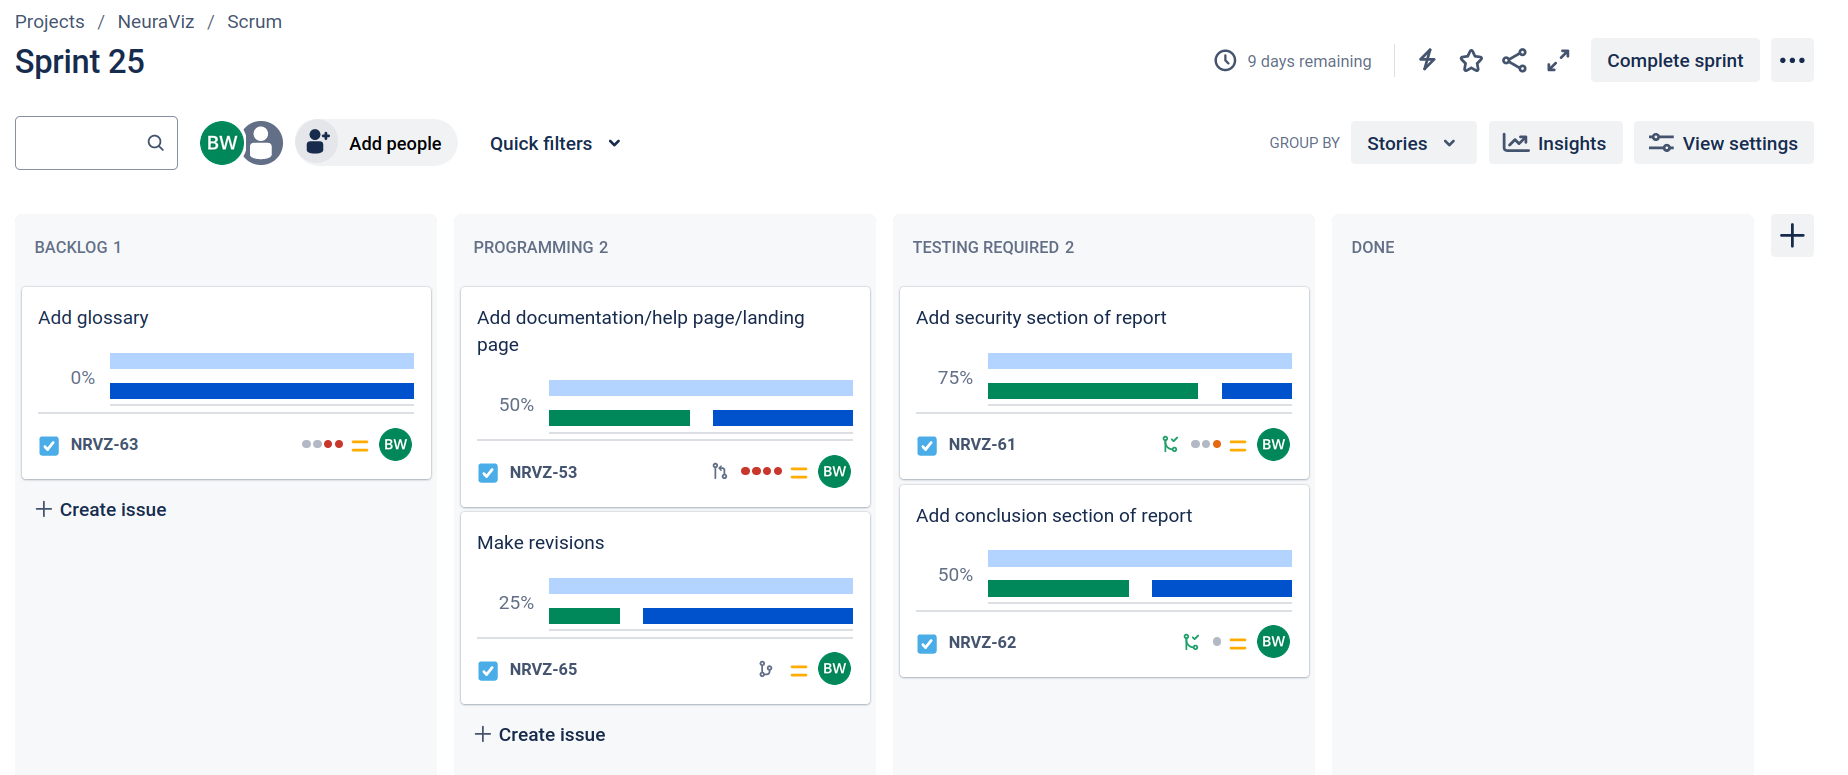
\includegraphics[width=1\textwidth]{02_dev_process/res/jira_board_sprint_25.png}
    \caption[Jira Scrum Board]{Jira Scrum Board}
    \label{fig:jira_scrum_board}
\end{figure}

In addition to Jira, Github was used to help keep track of individual sprint tasks using separate feature branches. A new branch was created for each task, with the name of the branch including the task key from Jira and a brief description. Jira's integration with GitHub provided a link to see what development phase the code was in directly from the Jira task, including whether a pull request had been created or merged.

\subsection{Functional Requirements}
Because agile methodologies were chosen for the development of this project, a set of functional requirements in the form of user stories were collected prior to the start of development. These user stories served as a guide for features to implement and helped ensure that no major functionality was missed during development.

NeuraViz is a relatively simple application with only one type of user. As such, the functional requirements are relatively straightforward, including the ability to upload a pre-trained machine learning model trained in either PyTorch or Keras. In addition, users should be able to see either the full graph of the uploaded model, or a collapsed version depending on the scale of the uploaded model. Additional functionality is also documented such as the ability to navigate the page via pan and zoom functionality on the graph and being able to click or hover on various network components. 

In addition to the functionality of viewing the network itself, user stories were also documented for export functionality, allowing the graph of the model to be exported both as an SVG and as a \LaTeX{} document in the format of a TikZ picture. 

The full set of user stories is documented in \href{https://github.com/Bennett-Wendorf/NeuraViz/blob/main/docs/user_stories.md}{the user stories document} found in the ``docs'' directory of the Github repository. This document also includes user stories for functionality that was not implemented in the current version of NeuraViz but may be implemented in future versions.

\subsection{Non-Functional Requirements}
In addition to the functionality documented as user stories, non-functional requirements were also documented to ensure that the user experience of NeuraViz was as smooth as possible. Identified non-functional requirements are as follows:
\begin{itemize}
    \item Large network layers are collapsed if they are too big to reasonably render.
    \item For visually impaired users, aria labels exist for screen readers where possible.
    \item If a page takes a long time to load, skeletonized components are shown to indicate that the page is still loading.
    \item As a user, my data is reasonably secure, both during transmission and processing.
    \item Themes are sufficiently differentiable for colorblind users.
    \item Invalid models are rejected and not stored on the server unnecessarily.
\end{itemize}
}{}\clearpage
\IfFileExists{03_design/design}{\section{Design}
\label{sec:Design}

\subsection{Overview} 
NeuraViz follows a fairly standard server-client web application architecture. The client is responsible for rendering the user interface and allowing the user to interact with the application. The server handles the actual computationally intensive processes such as parsing the uploaded model and generating the structure of the visual representation. The server also handles the storage of the uploaded models during user sessions. It also handles translation of the visualization into various formats.

\subsection{UML Class Diagram}
The UML class diagram in Figure \ref{fig:uml_class_diagram} shows the classes and their relationships in the NeuraViz application. The diagram is divided into two main sections: the frontend and the backend, which are also commonly referred to as the client and server respectively. 

\begin{figure}[h]
    \centering
    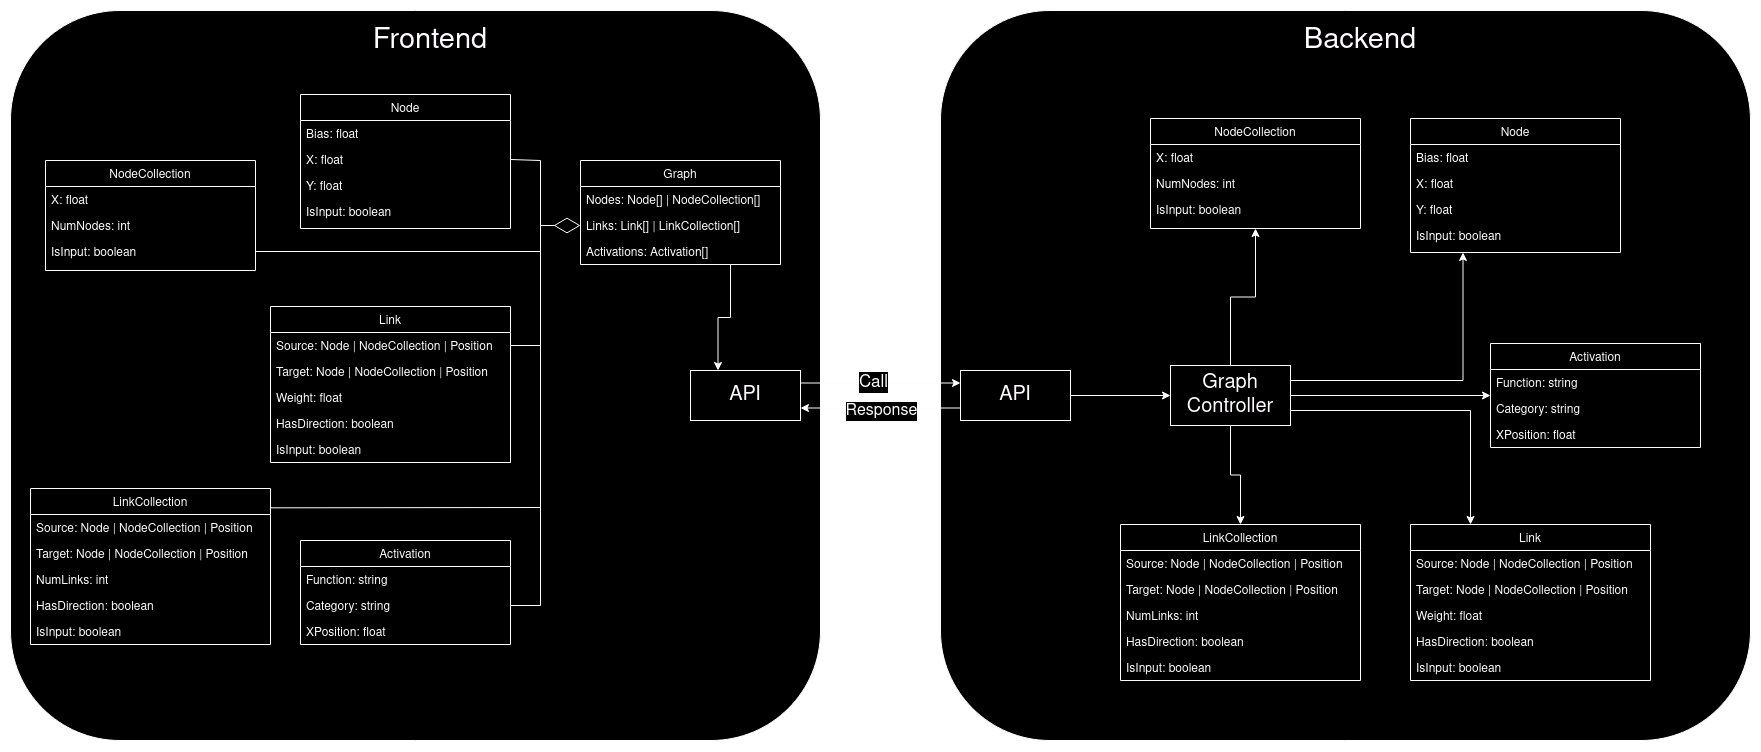
\includegraphics[width=0.8\textwidth]{../docs/diagrams/class_diagram.png}
    \caption{UML Class Diagram}
    \label{fig:uml_class_diagram}
\end{figure}

\subsubsection{Frontend/Client}
The frontend primarily relies on the Graph object, which is comprised of a number of Nodes and/or Node Collections, Links and/or Link Collections, and Activation Functions. Nodes represent individual nodes as represented in the graph, and these are used for nodes in graph layers that are smaller than 10 nodes by default. For layers that are too large, the graph representation instead contains a Node Collection that represents the layer as a whole. Links and Link Collections operate a similar way. Activation Function objects represent the activation functions that can be seen as small icons at the top of each layer in the NeuraViz interface. The graph object houses the representation of the neural network model as ready for rendering. As shown in the UML diagram, the frontend also houses an API component that is responsible for communicating with the backend architecture via standard HTTP requests.

\subsubsection{Backend/Server}
The backend is responsible for handling the computationally intensive processes of parsing the uploaded model and generating the structure of the visual representation. As seen in Figure \ref{fig:uml_class_diagram}, the backend houses objects that almost perfectly mirror the frontend components. However, on the server, these components are all related to the graph controller: the component responsible for the actual graph parsing. In addition to parsing the actual graph, the controller also handles additional requests for retrieving a stored model and converting the representation into various formats. Like with the frontend portion of the application, the backend houses an API component that is responsible for receiving the HTTP requests from the client and routing them to the correct controller endpoint for processing, as well as sending the response back to the client.

\subsection{Database}
% TODO: Add Database

\subsection{User Interface}
% TODO: Add User Interface
}{}\clearpage
\IfFileExists{04_implementation/implementation}{\section{Implementation}
\label{sec:Implementation}

\subsection{Technologies Used}
NeuraViz was developed with a multitude of standard web technologies used in conjunction to build the classic client-server architecture that was settled on. The chosen technologies were used for their stable and well-documented nature, as well as their ability to interact with libraries and frameworks specific to neural networks. This section describes what technologies were used for each of the three constituent components of NeuraViz.

\subsubsection{Client}
The client component is the primary interface that the user acts with, and therefore must be visually appealing and responsive. In researching available web frameworks for building frontend web applications, a number of possibilities were considered including ReactJS, Angular, and Svelte. While ReactJS would have been a good choice for its popularity and the developer's experience, Svelte was eventually chosen for its simplicity and performance. 

Svelte \cite{svelte} is a relatively new web framework that is similar to ReactJS in that it is component-based, but it is different in that it compiles the components into vanilla JavaScript at build time. This means that the final product is much smaller and faster than a ReactJS application, which must include the React library in the final product. Svelte also has a simpler syntax than ReactJS, which makes it easier to learn and use. In particular, Svelte's feature set across reactivity of its components, ease of implementing special features such as animations, and built-in global store system turned out to be especially helpful during the development of NeuraViz. Svelte also natively supports TypeScript, a superset of JavaScript that introduces a strong static type system and a powerful type inference system that helped keep the codebase clean and maintainable, while still providing the freedom to work in a web environment seamlessly.

Though Svelte is a powerful and featureful framework on its own, two shortcomings were identified during NeuraViz's development that had to be overcome with additional libraries. Svelte's component system does a fantastic job of abstracting components into small, reusable pieces, but it lacks prebuilt components that would keep the application's look and feel consistent and the development rapid. To remedy this problem the Flowbite Svelte library \cite{flowbite} was used. Flowbite provides prebuilt Svelte components that fulfill many of the necessary functionalities of a web application. For example, it contains components such as buttons, text boxes, dialogs, and more. Being built on top of TailwindCSS \cite{tailwind}, Flowbite also provides excellent support for light and dark application themes. As its second shortcoming, Svelte does not include functionality for sending or receiving HTTP requests. While JavaScript's native fetch function would work for this, Axios \cite{axios} provides a much cleaner experience for handling HTTP calls and responses. Axios also provides support for handling the asynchronous nature of HTTP requests via JavaScript's promise API and callback functions.

Graph visualization, being the most critical feature of NeuraViz, was a major consideration when determining client technologies. To aid in the construction of the graph visualization, the D3.js library \cite{d3} was used. D3 is a highly customizable JavaScript library for creating visualizations of data in all different formats. It works by providing abstractions on the DOM for building SVG elements easily and dynamically. In addition to providing methods for creating large numbers of static SVG elements, D3 also contains abstractions for dealing with animations and movement such as the functionality in NeuraViz for dragging the graph around and zooming in and out. The modular nature of the library also makes it perfect for dealing with the programmatic generation of complex visualizations such as those necessary in this project.

\subsubsection{Server}
When deciding what programming language to use for the server side of NeuraViz, a major consideration was the integration with the uploaded neural network models and the complexities of parsing them. The eventual decision was that it would not just easier, but also more maintainable to include the libraries themselves and then extract the necessary information from the objects rather than parsing the model files manually. Since most popular machine learning frameworks are written for Python, it made sense to write NeuraViz's server in Python as well. 

To accommodate this language choice fully, Quart \cite{quart} was selected for managing the server side of the application. Quart is a partial rewrite fo the popular Python web framework Flask, with support for asynchronous operations baked in. In NeuraViz, Quart is simply used as an API manager and to serve the static frontend compiled with Svelte, though it does have support for compiling and serving the HTML, CSS, and JS necessary to run a web application itself. Managing an API in Quart is as simple as defining async handler functions and adding Quart's decorator to specify what route should call that function. While the parsing operations are complex, the number of endpoints that this API requires is relatively small. Table \ref{tab:api_endpoints} shows the full list of routes that the server provides.

\begin{center}
    \begin{tabular}{|l|l|}
        \hline
        \rowcolor{gray!40} Endpoint & \textbf{POST /graph} \\
        \hline
        Description & Upload the graph model and retrieve the intermittent representation. \\
        \hline
        Inputs & The graph model as a file in the request \\
        \hline
        Responses & 200 OK - Graph representation is returned \\
        & 400 Bad Request - The file was not valid \\
        & 501 Not Implemented - The file type is not supported \\
        \hline
        \rowcolor{gray!40} Endpoint & \textbf{GET /tikz}\\
        \hline
        Description & Retrieve the session's graph as a \LaTeX{} file using Tikz (in light mode) \\
        \hline
        Inputs & None \\
        \hline
        Responses & 200 OK - \LaTeX{} is returned as a string \\
        & 400 Bad Request - No graph was found in the session \\
        \hline
        \rowcolor{gray!40} Endpoint & \textbf{GET /tikz/dark} \\
        \hline 
        Description & Get the dark mode version of the Tikz representation \\
        \hline
        Inputs & None \\
        \hline
        Responses & 200 OK - \LaTeX{} is returned as a string \\
        & 400 Bad Request - No graph was found in the session \\
        \hline
    \end{tabular}
    \captionof{table}{Server API Endpoints}
    \label{tab:api_endpoints}
\end{center}

Currently, NeuraViz supports visualizing models creating with Keras and Pytorch. As such, both of those frameworks are also included in the server of the application. When the graph endpoint is hit, the correct framework is determined based on the file extension of the uploaded file From there, the framework is used to decode the model into a Python object and that Python object is then parsed to retrieve the information needed for NeuraViz's visualization.

\subsubsection{Data Layer}
NeuraViz has a relatively simple data layer as the only persistent data is session information. Due to this simple nature, MongoDB \cite{mongodb} was decided on for storing the data. Mongo is a NoSQL database implementation that Python has good support for through the PyMongo package \cite{pymongo}. Models were written for each of the constituent parts of the stored graph as well as for the session itself. A custom module was also written for managing the sessions to encourage session management to happen for each API endpoint.

\subsection{Development}
The development of NeuraViz was completed over the course of 22 one-week long sprints. The first two sprints comprised primarily of designing the application. Sprints 3-10 focused on building the main functionality of the application for models uploaded with Pytorch. The remaining sprints added Keras support and additional features.
% TODO: Update sprint count

Design work on the application began by thinking through a set of desired features. Since NeuraViz isn't built for a particular client, this primarily consisted of the developer coming up with ideas and those ideas being vetted by the project advisor to come up with a final concept for the project. Once there was a solid understanding of at least the basic functionality that the application would fulfill, a user interface mockup (see Figure \ref{fig:ui_mockup}) was created to give a visual representation of what the application would look like. This design step also served to iron out some flaws before development on the actual application began. The UI mockup was heavily referenced when creating the actual application UI, and the final product is very similar to what the mockup originally showed.

Once the design was ready, development began. The first step was learning the two new frameworks (namely Svelte and Quart) and working to get them integrated with each other. The developer had previous experience with ReactJS, so Svelte's similar structure made the learning curve relatively small, and the concepts were picked up quickly. With experience building web application backends, Quart was also relatively easy to pick up and get working. The first few sprints after design were spent getting these two frameworks set up, laying out the basic structure of the frontend and following the mockups by following the mockups, and setting up the backend to serve the compiled frontend and handle the necessary API endpoints.

After the basic structure of the application was in place, the next step was figuring out how to use D3.js to create the visualization of the graph. Since the server-side graph parser had not been completed at this point, the graph structure was hard-coded in the application to allow for quick iteration on what the data needed to look like for the visualization to work and be as easy as possible to transmit across the network. An additional major step in this process was getting the pan and zoom functionality of the graph visualization working properly. While D3 provides some of the functionality, getting it working in the way that NeuraViz needed was a significant challenge that required a lot of trial and error.

The next major step was getting the server to parse the uploaded model files. This was a significant challenge as the structure of the model files is complex and not well documented. Because of this complexity, it was decided to let the frameworks parse the models themselves, and to extract the necessary information from the objects that the frameworks produced. While this cut out some of the complexity of trying to parse the files the frameworks produce, it still maintained the complexity of dealing with the object-oriented representation of the objects in Python. Most machine learning frameworks expect developers to build, train, and execute models through their frameworks, but parsing those models out to alternative representations is generally not an intended use-case. Because of this, documentation on how the objects are structured and exactly where the necessary information is stored is sparse. An extensive amount of time was required to investigate the object structure in each framework and determine how that information can be converted into NeuraViz's standardized representation. To speed up this process, Pytorch alone was focused on at first, and then support for Keras models was added later.

Once server support for parsing Pytorch models and frontend graph visualization were complete, additional features could be added to further enhance the application. Some of the more useful additional features included adding support for activation function representations on the graph, exporting the visualization to \LaTeX{} or SVG, and color-coding model parts to indicate more information at a glance. These features were added toward the second half of the development process.

\subsection{Deployment}
Being a web application, deployment of NeuraViz is a complex process that involves multiple steps. The first step is to compile the Svelte frontend into static HTML, CSS, and JavaScript files. This is done by running the command \texttt{npm run build} in the frontend directory. This command compiles the Svelte code into a set of static files that can be served by a web server. The next step is to copy these files into the server directory so the backend portion of the application can serve up these files. The final step is to start the Quart server, which listens for incoming requests on port 5000 by default. Once the server is running, the application can be accessed by navigating to \texttt{http://localhost:5000} in a web browser.

% TODO: Add some detail about prelim research on frameworks
% TODO: Add detail on how I use the frameworks to parse

However, running the the application on localhost does not make it available the internet as a whole. To make the application accessible to the public, it was deployed to a private web server and routed from \href{https://neuraviz.bennettwendorf.dev}{https://neuraviz.bennettwendorf.dev}. The private server runs Ubuntu and PM2 \cite{pm2} was used to help manage the process and allow it to automatically restart when the server restarts.

To speed up deployment to the server, Github Actions was used to automatically build and deploy the application whenever a new commit was pushed to the main branch. The action itself works by setting up a vpn connection to the server and using SSH to run a script on the server. The action configuration is shown in Listing \ref{lst:action_config}.

\begin{center}
    \lstinputlisting[caption={Github Action Configuration}, label={lst:action_config}, float=htb, language=yaml]{../.github/workflows/deploy.yml}
\end{center}

The referenced build script begins by pulling new changes from the remote Github repository. It then cleans all old build files to ensure that everything gets rebuilt fresh. Once the environment is clean, it ensures that all project dependencies are up to date on the server, and installs any new ones if needed. It then recompiles the Svelte frontend and copies it into the necessary location in the backend. Finally, the script uses pm2 to restart the server and serve the new version of the application.
% TODO: Include build script as appendix}{}\clearpage
\IfFileExists{05_testing/testing}{\section{Testing}
\label{sec:Testing}

\subsection{Overview} 
Per the scrum software design process, software verification and validation were performed continuously throughout development. To accommodate this and ensure that thorough testing was performed, a \textit{Testing Required} status column was added to the scrum board. Once sprint tasks finished development, they were moved to this column to ensure that testing was completed before the sprint task was considered complete.

\subsection{Unit Testing}
During development, a large amount of unit testing was created and performed to support the continuous and thorough testing process that was defined at the outset of the project. Due to the small size of the development team, test cases were both written and executed by the developer. Test processes that were used during the development of NeuraViz can be broken down into two major categories: frontend or client testing and backend or server testing. In total, 31 automated test cases and 10 manual test cases were written and executed for the application. A one hundred percent pass rate was achieved before each sprint task was considered complete.

\subsubsection{Frontend Testing}
The frontend of NeuraViz was tested using a combination of automated and manual unit testing. Testing a user interface is a challengep primarily due to its visual nature, but tools exist to help automate this process. For this application, the automated testing platform Playwright \cite{playwright} was used to develop test cases that could be executed against each individual sprint task and at any time. Automated testing in this manner is especially useful to ensure that test cases are performed both consistently and repeatably, with minimal human error. 

Playwright test cases work by defining actions that should be taken in the user interface, and asserting various results. These results can include a variety of things, such as the presence of certain elements on the page, that a certain number of elements exist, or text on an element. Test cases are written directly in JavaScript and by default run in an automated headless browser so as not to interfere with other work that is being done. An example of a test case that was written for NeuraViz is shown in Listing \ref{lst:playwright-example}. This test case ensures that clicking the model upload button with no model file selected leads to the validation text staying red and saying ``Model is not valid''. On line 3 an example can be seen of an action being taken; in this case, the button with the name ``Upload'' is clicked. On lines 4-6, assertions are made about the state of the page after the action is taken.

\begin{center}
    \begin{lstlisting}[language=JavaScript, float=*htb, caption={Playwright Test Case Example}, label={lst:playwright-example}]
    test('Upload no model: Sidebar', async ({ page }) => {
        await page.goto('/');
        await page.getByRole('button', 
            { name: 'Upload' }).click();
        await expect(page.locator('#model-upload'))
            .toHaveValue('');
        await expect(page.locator('#model-validation'))
            .toHaveText('Model is not valid');
        await expect(page.locator('#model-validation'))
            .toHaveClass(/text-error/);
    });
    \end{lstlisting}
\end{center}

\subsubsection{Backend Testing}
Like the frontend, NeuraViz's backend code was also tested using a mix of automated and manual unit testing. While most of the functionality could easily be tested automatically, features such as SVG and TikZ export need to be inspected visually, and so were included in manual testing rather than automated testing. As with the frontend, as much functionality as possible was tested automatically to reduce the overhead in maintaining a test suite and to further enforce a continuous testing process. The backend automated test suite was developed with the Python testing framework Pytest \cite{pytest}. This framework allows for the easy definition of test cases and the execution of those test cases in a repeatable and consistent manner. An example of a test case that was written for NeuraViz is shown in Listing \ref{lst:pytest-example}. This test ensures that the JSON representation of an uploaded model matches what is expected, specifically for the PyTorch Iris model. The test case first uploads the model with Quart's test client, then asserts that the result exactly matches the expected result.

\begin{center}
    \begin{lstlisting}[language=Python, float=*htb, caption={Pytest Test Case Example}, label={lst:pytest-example}]
    @pytest.mark.asyncio
    async def test_get_graph_nominal_pytorch_iris(self) -> None:
        test_client = app.test_client()
        file_name = "STE_Iris.pth"
        files = {
            'files[]': FileStorage(stream=open(f"testing/input_files/pytorch/{file_name}", 'rb'), filename=file_name)
        }
        response = await test_client.post('/api/graph/', files=files, headers={'Content-Type': 'multipart/form-data'})
        assert response.status_code == 200
        data = await response.get_json()
        with open("src/backend/tests/expected_results/get_graph/pytorch/nominal_STE_Iris.json", 'r') as file:
            expected_data = load(file)
            assert data == expected_data
    \end{lstlisting}
\end{center}

\subsection{Regression and Integration Testing}
Regression testing during the development of NeuraViz was handled implicitly during the test phase on each individual sprint task and before that sprint task was merged and considered complete. During this phase, new test cases were written for the feature. Once written, these test cases along with all existing automated test cases were executed to ensure that nothing new or old contained a regression. In addition, manual test cases were investigated to ensure that the new feature did not break any existing functionality. To further ensure that the product remained stable, test cases were also run before each version release and publication to the production server.  

While unit tests can only really cover functionality on the frontend or backend, testing was also performed during feature development and periodically to ensure that the features all worked together seamlessly. This was done by running the application and testing a feature from start to finish, typically referred to as end-to-end testing. This type of testing was also performed extensively before the release of each version to the production server.}{}\clearpage
\IfFileExists{06_security/security}{\section{Security}																	
\label{sec:Security}

\subsection{Overview} 
NeuraViz does not store user information long-term in any capacity, so security of data storage was not a major point of concern during development. However, it is feasible that users might upload proprietary models to the system, and so the security of information during transportation was an important consideration during development. Steps taken to combat security threats are outlined in this section.

\subsection{Web Application Security}
Web applications are inherently vulnerable due to their constant communication of data across the internet and the fact that the client has access to the client-side source code. For NeuraViz, this is less of an issue than other applications because the user is not modifying any stored data on the server that could potentially be corrupted by malicious data. However, precautions were still taken to ensure that the application is secure.

NeuraViz is hosted over HTTPS, which encrypts all data sent between the client and server via the Transport Layer Security (TLS) protocol. This ensures that data is not intercepted or tampered with during transit. In production, NeuraViz is hosted on a dot dev domain, which enforces HTTPS by default, completely disabling users from connecting over unsecure HTTP. In addition, the production application is hosted on a secure private server with a certificate provided by Let's Encrypt \cite{letsencrypt}, which is a free, automated, and open certificate authority. This certificate is used to verify that the server is who it claims to be, and is used to encrypt the data sent between the client and server, providing the user with additional peace of mind when using the application.

Because this project does not take any user input directly, the risk of cross-site scripting attacks or other similar threats related to input sanitization is minimal. However, there is still some risk in the retrieval and storage of uploaded models from the user. To protect the application server itself, uploaded files are never executed directly. Upon upload, the file is stored temporarily on disk and the corresponding model framework is used to parse the file contents, based on the file extension. Because all supported frameworks are open source and well tested, the security of their file parsing is very likely to be robust and secure. If the framework encounters an issue during parsing such as an invalid portion of the file, the file is deleted from disk and the user is notified of the error. Both PyTorch and Keras store their models in a binary object format which contains no executable code. Once the file is parsed by the framework, NeuraViz uses the respective framework's own Python objects to generate the representation of the model, again with minimal execution of third-party code. Throughout this process, NeuraViz is very particular about the kind of data it expects from the model, and will quickly fail if the data is not as expected. This practice of essentially white-listing valid data also helps prevent any unexpected behavior from the application that could negatively impact user experience or security.

\subsection{Session Management}
To accommodate an elevated user experience, NeuraViz stores session data in a MongoDB database on the server. The stored session information consists of a session identifier, the full representation of the model in a similar format to what is returned to the user after uploading a file, and a timestamp. The session identifier is a randomly generated string that is unique to each session, and as such is not tied to a particular user in any way, making it nearly impossible to associate a stored model with a particular user other than by the session token itself. The session identifier is stored as a cookie by the client and can be used to retrieve the stored model for the duration of the session. To mitigate possible security risks, the database is only accessible from the server where the application is running. Furthermore, while the server is running, sessions are automatically pruned after 10 minutes of inactivity. This trade-off allows the user to continue making requests without the application needing to parse the model again, while providing a reasonable level of security for the stored model.
}{}\clearpage
\IfFileExists{07_conclusion/conclusion}{\section{Conclusion}																	
\label{sec:Conclusion}

\subsection{Overview} 
The NeuraViz project has successfully accomplished all of its primary goals in creating a user-friendly web application for visualizing artificial neural network architectures. It provides its users with the capability to upload pre-trained models from both Pytorch and Keras, visualize their structure, and export the visualizations to both SVG and LaTeX.

\subsection{Challenges}
A number of challenges and roadblocks were encountered throughout the development process, including a large amount of research into each framework, and personal time management. Each of the machine learning frameworks used have complex internal data structures that they use to model neural networks and be able to run inferences and training on them. However, these data structures are generally only designed to be used internally, and are not well documented for external use. In addition, because neural network training and inferencing is complex, the objects used by the frameworks often contain a large amount of information that is not relevant to the visualization, and must be filtered out. To develop NeuraViz's parsing algorithm, extensive research was required to understand the internal data structures that are used by Pytorch and Keras, and determine where necessary common information could be extracted to produce a cohesive experience for the user, regardless of how they chose to create their model in the first place.

As with many projects, time management was a constant struggle. Balancing development of NeuraViz with other obligations, whether school, work, or personal, was a significant hinderance to the rate of development that could be performed on this project, and ultimately limited the feature set that was able to be completed. However, it was known at the outset that many of the goals of this project were extensive and would likely not be fully completed within the time frame of the project.

\subsection{Future Work}
Throughout the planning and development of this project, a number of additional potential features were identified that could be added to NeuraViz to improve its functionality and usability. These include additions such as adding support for more model types, visualizing more complex networks like recurrent or convolutional networks, and animating the visualization to show the flow of data through the network.

While Pytorch and Keras cover a substantial portion of the industry for creating, training, and deploying neural networks, there are a multitude of other frameworks that are used in various industries. To fully realize the potential that NeuraViz provides, ideally every major framework would be supported, allowing users to visualize their models in a consistent manner regardless of their chosen framework. This would require extensive research both into what frameworks are used in industry, and the exact internal structures they use to model neural networks. On top of that, maintaining the tool with the ever-increasing number of products on the market would be a monumental task. Hopefully with NeuraViz being open source and freely available, more developers will be able to contribute and help expand this list. 

Visualizing more complex network types was one of the initial goals of this project. However, development tended more toward a use-case in an educational environment, rather than professional. While recurrent and convolutional networks are still beneficial to teach, they are more complex and not as often taught in an academic capacity, and therefore were left out of the project. However, adding support for these types of networks would drastically increase the utility of NeuraViz's major function of providing a consistent representation of many different types of neural networks. 

With the tendency more toward education during this project's development, the ability to animate data through a smaller network would be a great addition. An instructor could show a visualization to a class, and step through each step of the inferencing process live, instantly seeing how changes in the input data affect the output. Implementing a feature like this would take a significant amount of work, so it was left out of the project scope for the time-being.}{}\clearpage

%% BIBLIOGRAPHY
\bibliographystyle{plain}
\bibliography{bibliography}
\clearpage

%%% APPENDICES
\section{Appendices}
\label{sec:appendices}
\clearpage

\end{document}
